\documentclass{llncs}

\usepackage{amssymb}
\setcounter{tocdepth}{3}
\usepackage{graphicx}
\usepackage[table,xcdraw]{xcolor}
\usepackage[ruled]{algorithm2e}
%\usepackage[lined,boxed,commentsnumbered]{algorithm2e}
\usepackage{amssymb}
\usepackage{amsmath,graphicx,color,doi}
\usepackage{algorithm2e}
%\usepackage{algorithmic}	
\usepackage{multirow}
\usepackage{subfigure}
\usepackage{cite}


\newcommand{\gi}[1]{{\textcolor{red}{[\small \textbf{Giacomo}: #1]}}}
\newcommand{\ad}[1]{{\textcolor{red}{[\small \textbf{Adriano}: #1]}}}
\newcommand{\cl}[1]{{\textcolor{red}{[\small \textbf{Claudio}: #1]}}}

%\newcommand{\gi}[1]{}
%\newcommand{\ad}[1]{}
%\newcommand{\cl}[1]{}


\begin{document}
\title{Tampering Detection In Low-Power Smart Cameras}

\author{Adriano Gaibotti\inst{1,}\inst{2} \and Claudio Marchisio\inst{1} \and Alexandro Sentinelli\inst{1} \and \\ Giacomo Boracchi\inst{2}}

\institute{ 
	STMicroelectronics, Advanced System Technology, Via Camillo Olivetti 2, 20864, Agrate Brianza (MB), Italy\\
	\email{\{adriano.gaibotti, claudio.marchisio, alexandro.sentinelli\}@st.com}
	\and
	Politecnico di Milano, Dipartimento di Elettronica, Informazione e Bioingegneria (DEIB), Via Ponzio 34/5, 20133, Milano (MI), Italy\\
	\email{giacomo.boracchi@polimi.it}
}
\maketitle

\begin{abstract}
A desirable feature in smart cameras is the ability to autonomously detect any tampering event/attack that would prevent a clear view over the monitored scene. No matter whether tampering is due to atmospheric phenomena (e.g., few rain drops over the camera lens) or to malicious attacks (e.g., the device displacement), these have to be promptly detected to possibly activate countermeasures. Tampering detection becomes particularly challenging in battery-powered cameras, where it is not possible to acquire images at full-speed  frame-rates, nor use sophisticated image-analysis algorithms. 

We here introduce a tampering-detection algorithm specifically designed for low-power smart cameras: the algorithm leverages very simple indicators that are then monitored by an outlier-detection scheme. Any frame yielding anomalous indicator is detected as a tampered frame. Core of the algorithm is the partitioning of the scene into adaptively defined regions, that are preliminarily defined by segmenting the image during the algorithm-configuration phase, and which shows to improve the detection of camera displacements. Our experiments show that the proposed algorithm can successfully operate on sequences acquired at very low-frame rate, such as one frame every minute, with a very small computational complexity. %and leveraging the image partitioning into regions yields improved performance with respect to monitoring the whole scene
\keywords{tampering detection, blurring detection, displacement detection}
\end{abstract}



\section{Introduction}\label{sec:introduction}
% What is the problem?
When cameras operate outdoor and in harsh environments, dust, rain drops or snow flakes might lie on the camera lens resulting in blurry pictures, as shown in Figure \ref{fig:pioggia}, or in partial occlusions of the scene, as in Figure \ref{fig:neve}. Similarly, intentional attacks like displacing the camera, changing its focus, or spraying some opaque or glossy liquid over the lenses, would result in heavily compromised pictures, that would be useless for monitoring purposes. We refer to these events/attacks as tampering. In some cases, tampering is easy to detect, e.g., when the camera integrity is affected and the device goes out-of-order. However, in many other situations, namely when the device is not physically damaged, tampering detection is not straightforward, and sometimes image analysis is the only viable option. 

\begin{figure}[t!]
\centering
\subfigure[]{\label{fig:pioggia} 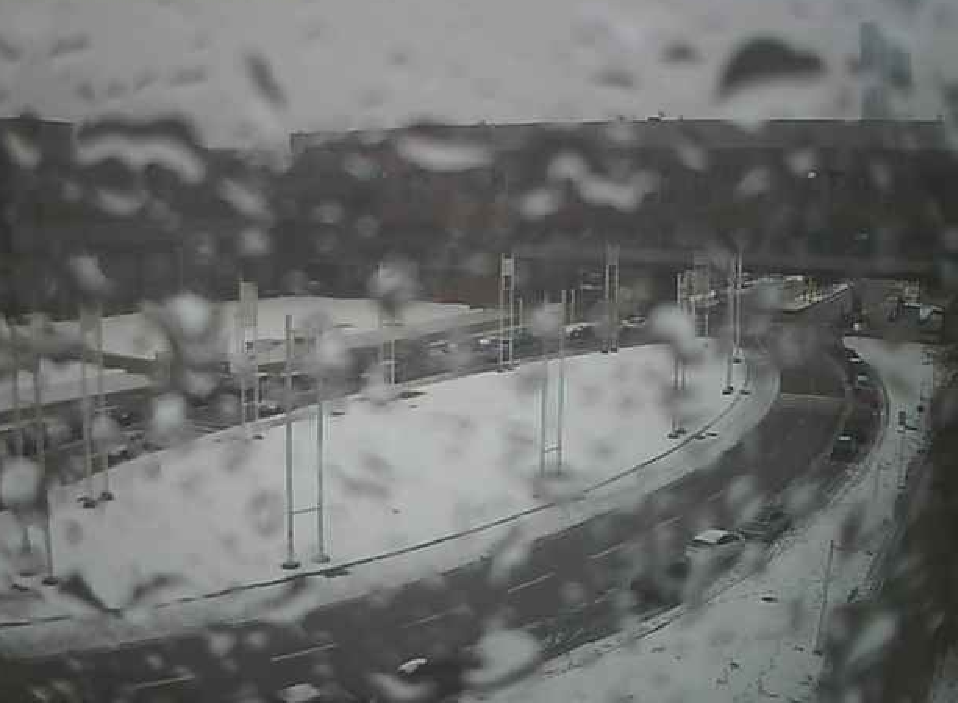
\includegraphics[width=0.225\linewidth]{Immagini/pioggia}}
\subfigure[]{\label{fig:neve} 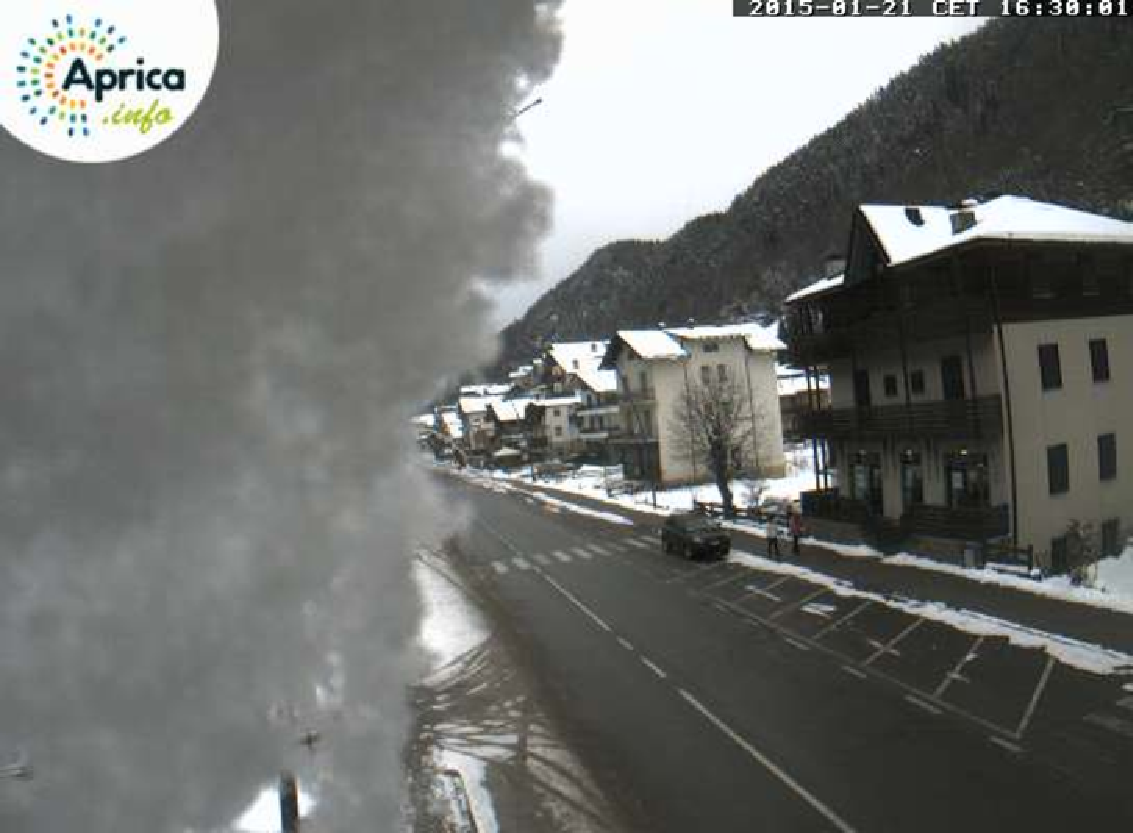
\includegraphics[width=0.225\linewidth]{Immagini/neve}}
\subfigure[]{\label{fig:displ1} 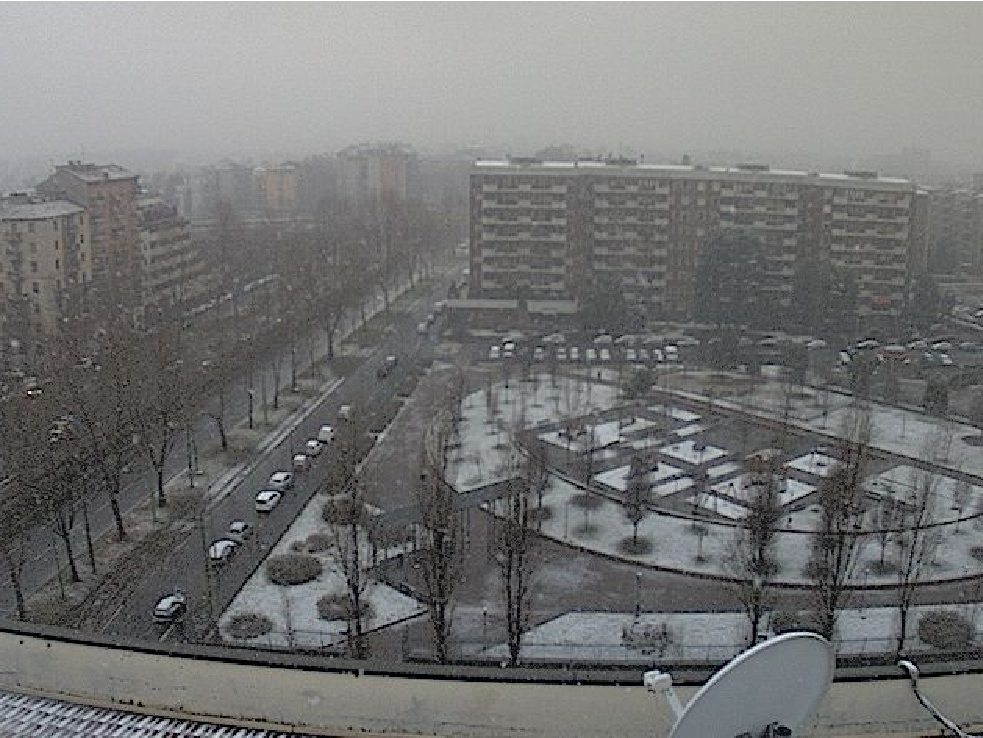
\includegraphics[width=0.225\linewidth]{Immagini/displ1}}
\subfigure[]{\label{fig:displ2} 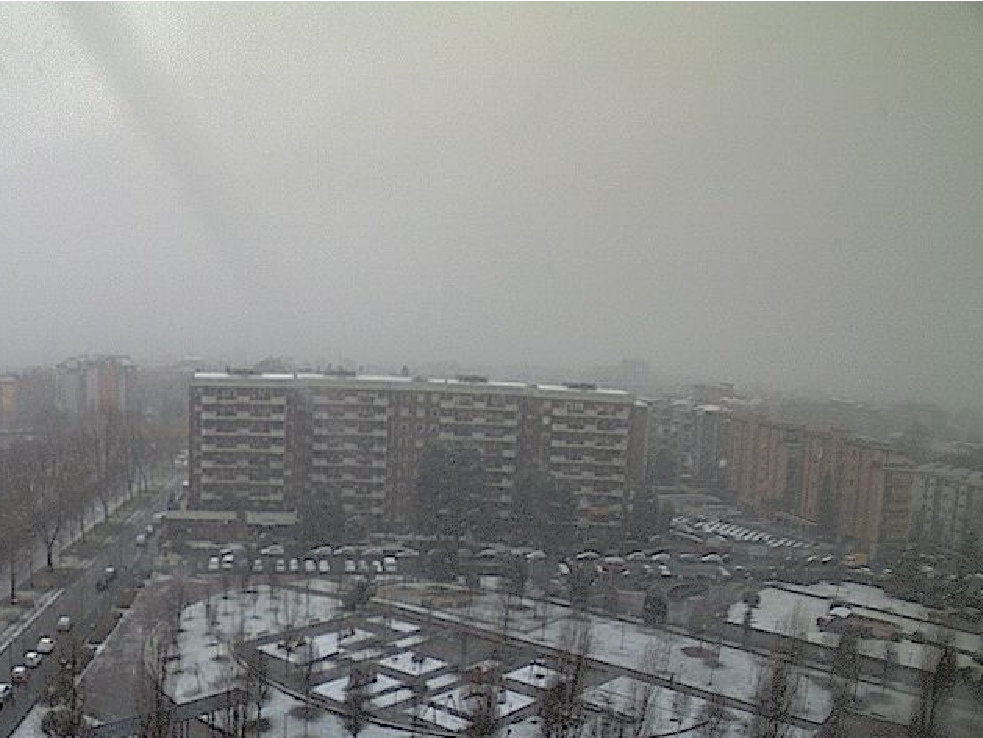
\includegraphics[width=0.225\linewidth]{Immagini/displ2}}
\caption[Tampering examples]{Examples of tampering events due to atmospheric phenomena. \textbf{(a)} Blur due to rain drops on the camera lens. \textbf{(b)} Occlusion due to snow on the camera lens.}
\label{fig:tampering}
\end{figure}

% Why is it interesting and important?
Tampering detection is an essential feature in surveillance systems~\cite{hampapur2005smart}, where cameras are expected to autonomously detect any tampering, and promptly report alerts. In fact, tampering prevents the correct interpretation of the scene: even a mild blur might hinder the identification of important details such as licence plates. Surveillance cameras are typically connected to the power supply and operate at normal frame-rates (e.g. around few frames per second): in these conditions, several tampering-detection algorithms have been presented. In particular, camera displacement and occlusions are typically detected by estimating the background or computing frame difference, while blurring is instead detected by monitoring the high-frequency components of images, as these are expected to drop. In~\cite{aksay2007camera} and~\cite{saglam2009real} tampering is detected by comparing histograms of background and current frame, and by monitoring the energy in wavelet or Fourier domain. Two background models, estimated over different time intervals, are used in~\cite{saglam2009real}. In~\cite{gil2007automatic}, tampering detection is performed by combining background subtraction together with edge detection and normalized cross-correlation. Background estimates and block matching in~\cite{tsesmelis2013tamper} enable the displacement detection, while the number of SURF~\cite{bay2006surf} keypoints is used to detect blurring. A frame buffer rather than an explicit background is used~\cite{ribnick2006real}. All these solutions, including~\cite{harasse2004automated,kryjak2012fpga} are computationally demanding, and are not viable options for low-power cameras. 

In this work we expressly target low-power and ultra-low-power smart cameras, like \emph{SecSoC} (Security System on Chip), an innovative prototype based on a cluster of ReISC (Reduced Energy Instruction Set Computer) cores, designed and producted by STMicroelectronics, operating at clock rates of 82.5 MHz at 1.2V and sub-1MHz at 0.6V. These devices are battery-powered, and characterized by a constrained computational power and memory availability. While low-power cameras are typically not employed in critical surveillance applications, they are becoming popular in distributed systems for monitoring wide environments due to their low cost and maintenance requirements.  %As an example, consider Wireless Multimedia Sensor Networks (WMSN) \cite{akyildiz2007survey} where smart-cameras can acquire and transmit images at regular time interval or upon requests. 
% These units are not connected to the power supply and have to operate with batteries and possibly rely on energy harvesting~\cite{magno2009adaptive}. 
%In practice, because of energy constrain, low-power devices have to operate at very low frame-rates: possibly less than one frame every minute.  

% Why is it hard? (E.g., why do naive approaches fail?)
Tampering detection in low-power smart cameras has not been much investigated in the literature~\cite{alippi2010detecting}, also because it is more challenging than in conventional surveillance cameras~\cite{perrig2004security}. Beside computational aspects -- such as the number of operations per pixels allowed -- the big issue is that low-power smart cameras typically operate at very low-frame rates (e.g., less than one frame per minute), thus the acquired sequence does not evolve smoothly. This prevents the use of learned background models and the analysis of foreground variations. In fact, when dynamic environments are acquired at low frame rates, two consecutive frames might be very different because of changes in the scene and in the light conditions, yielding sequences like those in Figure~\ref{fig:sequences}. Smart cameras have to promptly distinguish between \emph{normal} scene or illumination changes, and changes due to camera tampering to avoid the transmission of corrupted frames. Moreover, false alarms represent a serious problem in low-power smart cameras since they result in energy waste because of useless data processing and unnecessary network transmissions.
% We here address the problem of detecting tampering events on a camera device that is employed for monitoring purpose. Tampering events can be due to malicious attacks, as for instance a displacement of the camera or spraying some dirty liquid that would prevent the acquisition of (part of) the monitored scene or the interpretation of the content (e.g., the identification of licence plates). 

%What are the key components of my approach and results? Also include any specific limitations.
We address the detection of camera blurring and displacement, which are presented in Section \ref{sec:probForm}. The proposed algorithm, detailed in Section~\ref{sec:propSol}, relies on two indicators: the average image intensity is used to detect displacement, and the average gradient norm to detect blurring. These indicators can be easily computed and monitored by an outlier-detection technique in a low-power smart camera. In particular, we show that separately monitoring the indicators over different regions of the image can substantially improve the displacement-detection performance. Remarkably, these regions can be preliminarily defined during an initial configuration phase (Section \ref{subsec:Segmentation}), thus the algorithm operates at a negligible computational overhead w.r.t. monitoring the whole image (Section \ref{subsec:coputationalComplexity}). Thus, our solution represents a prompt trigger that can be possibly combined with other sequential monitoring techniques. Experiments in Section \ref{sec:experiments} show that leveraging image regions can substantially improve the displacement-detection performance. % Concluding remarks and discussions are given in Section \ref{sec:Conclusion}.

\begin{figure}[t]
\centering
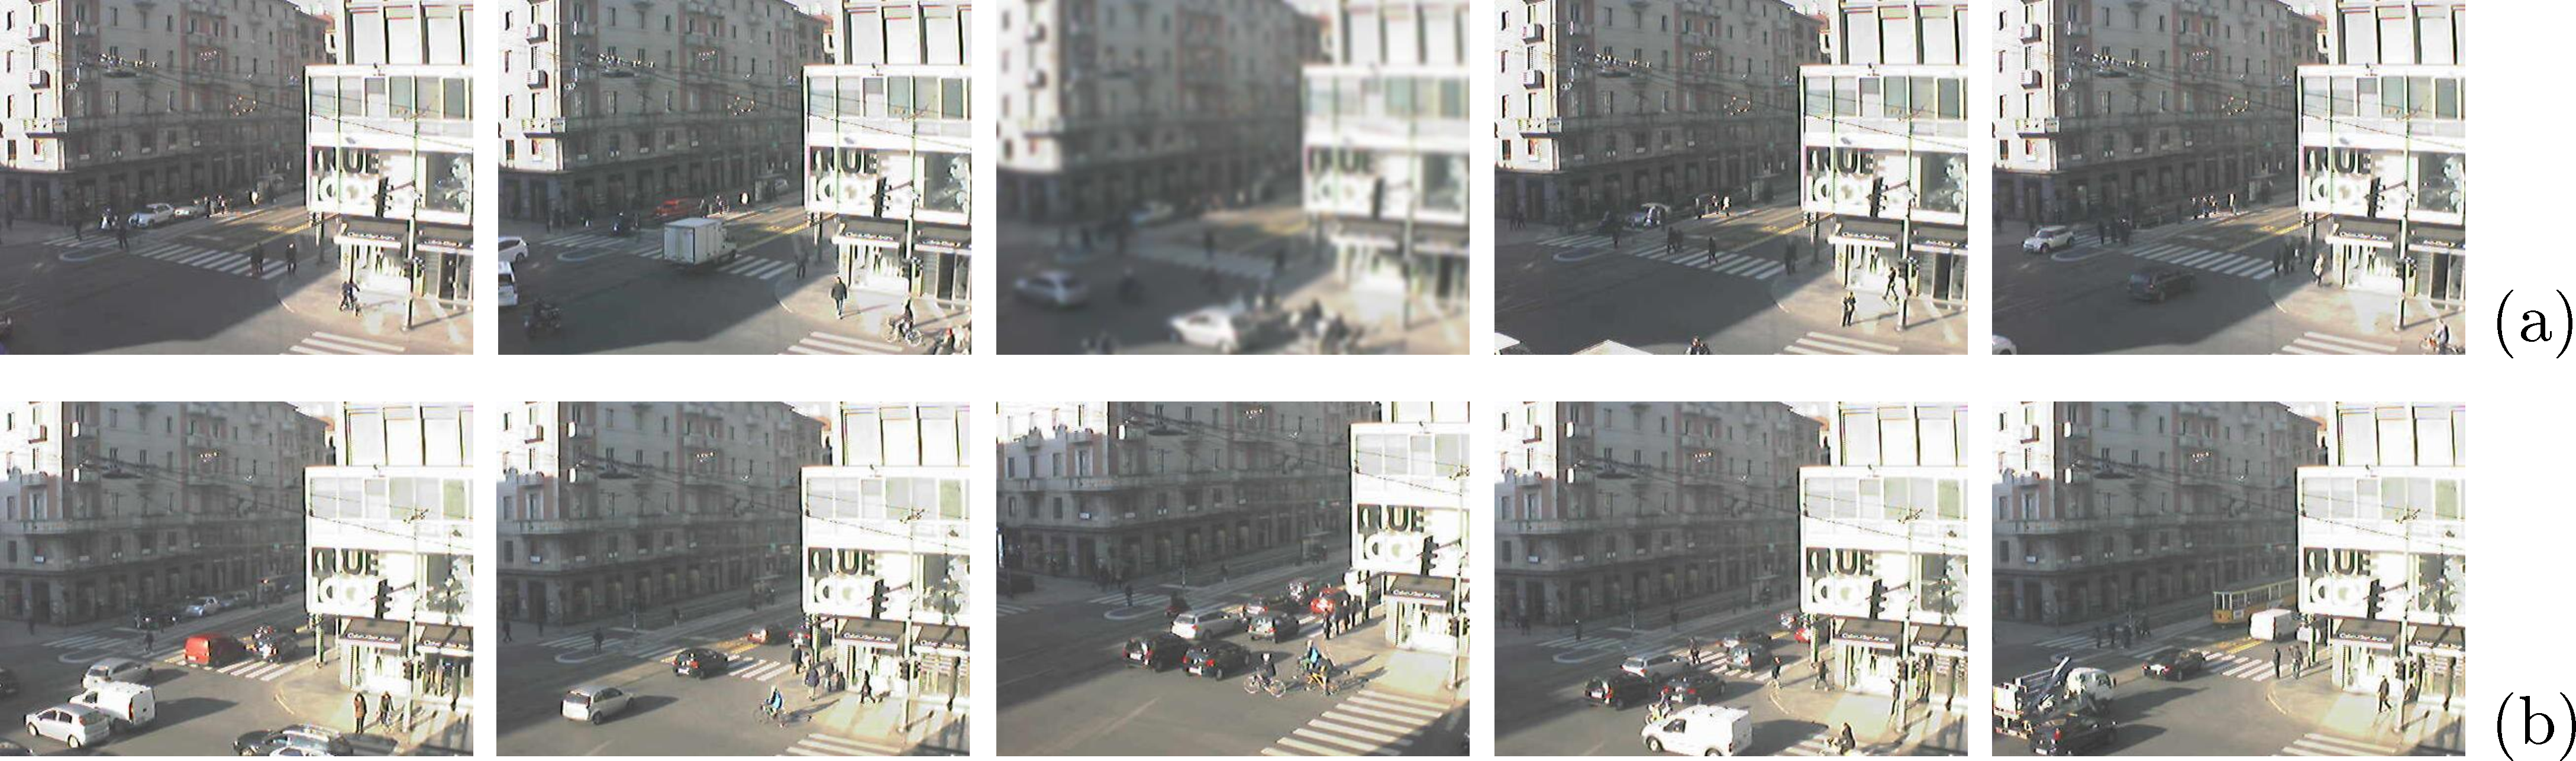
\includegraphics[width=1\linewidth]{Immagini/sequenze}
\caption{Sequences taken from webcams: \textbf{(a)} no tampering events; \textbf{(b)} defocus event on 3-rd frame, created using gaussian filtering; \textbf{(c)} displacement event on 3-rd frame, created moving the crop of the original image from the center.}
\label{fig:sequences}
\end{figure}


%A low-complexity and sequential monitoring scheme over the average gradient norm is used in~\cite{alippi2010detecting} to detect blurring due to external disturbances on the camera lens.

%\subsection{Related Works}\label{subsec:relWorks}
%% The literature concerning tampering detection is mostly focused on video surveillance applications and process at few frames per second.
% 
%%
%: comparison between frames belonging to a buffer in order to find high values of dissimilarity, associated to tampering.
%\cite{harasse2004automated}: tampering detection inside a moving vehicle; uses background subtraction methods in order to identify defocus, occlusions, and displacements. Comparison of edges pixels count for defocus detection, entropy comparison for occlusion detection, block matching algorithm for displacement detection.
%
%
%
\section{Problem Formulation}\label{sec:probForm}
%
Let $z_t$ be the frame acquired at time $t$
\begin{equation}
\label{eq:observationModel}
z_t(x)=\mathcal{D}_t[y_t](x) \quad \forall x \in X
\end{equation}
where $\mathcal{D}_t$ denotes an operator that transforms the original image $y_t$ in the acquired frame $z_t$; $X \subset \mathbb{Z}^2$ denotes the regular pixels grid and $x\in \mathbb{Z}^2$ indicates the pixel coordinates. As far as there are no tampering attacks/events,
\begin{equation}
\label{eq:no_tampering}
\mathcal{D}_t[y_t](x) = y_t(x) + \eta_t(x) \quad \forall x \in X
\end{equation}
where $\eta_t$ is a random variable accounting for image noise and $y_t$ are acquired from the same viewpoint and camera orientation, even though $y_t$ might show different content because of scene changes.\\
When, at time $\tau^*$, an external disturbance introduces \emph{blurring}, the image $y_t$ is degraded by an unknown blur operator, and $z_t$ becomes
\begin{equation}
\label{eq:model_defocus}
\mathcal{D}_t[y_t](x) = \int_{\mathcal{X}}y(s)h_t(x,s)ds\, + \eta_t(x) \quad \forall x \in X, t \geq \tau^*
\end{equation}
where $h_t(x,\cdot) > 0$ is the point-spread function at pixel $x \in X$.\\
A \emph{camera displacement} at frame $\tau^*$ is instead modeled as 
\begin{equation}
\label{eq:model_displacement}
z_t(x)  = \left\{ \begin{array}{rcl}
y_t(x) + \eta(x) & \mbox{per} & t < T^* \\
w_t(x) + \eta(x) & \mbox{per} & t \geqslant T^*
\end{array}\right. ,
\end{equation}
where $w_t$ relates to a different viewpoint and/or camera orientation than $y_t$. 

The proposed tampering-detection algorithm analyzes a sequence of frames $\{z_t\}_t$ to detect the time instant $\tau^*$ when tampering like \eqref{eq:model_defocus} or \eqref{eq:model_displacement} occurs. We assume that $T_0$ tampering-free frames are provided for training.

\section{Tampering Detection}\label{sec:propSol}

Algorithm~\ref{alg:DISPL} presents the proposed tampering detection, which relies on two simple indicators: the average intensity (also referred to as \emph{luma}, and denoted by $l$) and the average norm of the gradient (denoted by $g$). The former is meant to detect camera displacement, the latter image blurring since it causes a drop in the high-frequency content. As anticipated in Section~\ref{sec:introduction}, during the initial configuration, the scene is segmented in $K$ disjoint regions $\{R_k, k = 1,\dots,K\}$, namely $R_k \subset \mathcal{X}, R_i \cap R_j = \emptyset, \forall i \neq j$. The employed segmentation is detailed in Section~\ref{subsec:Segmentation}. 

For each $z_t$, the luma is separately computed within each of the $K$ regions:
\begin{equation}\label{eq:lumaRegions}
l_k(t) =\frac{1}{\#R_k} \sum_{x \in R_k} z_t(x), \ \ k = 1, \dots, K\,,
\end{equation}
while the average gradient norm is computed over the whole image
\begin{equation}
\label{eq:normaGradiente}
g(t) = \sum_{x \in X} \left (\sqrt{\left(z_t \circledast f_h\right)^2(x) + \left(z_t \circledast f_v\right)^2(x)}\right),
\end{equation}
where $f_h$ and $f_v$ are the horizontal and vertical derivative filters, respectively, $\circledast$ denotes the 2d convolution and $\#(\cdot)$ the cardinality of a set.

\begin{figure}[tb]
\centering
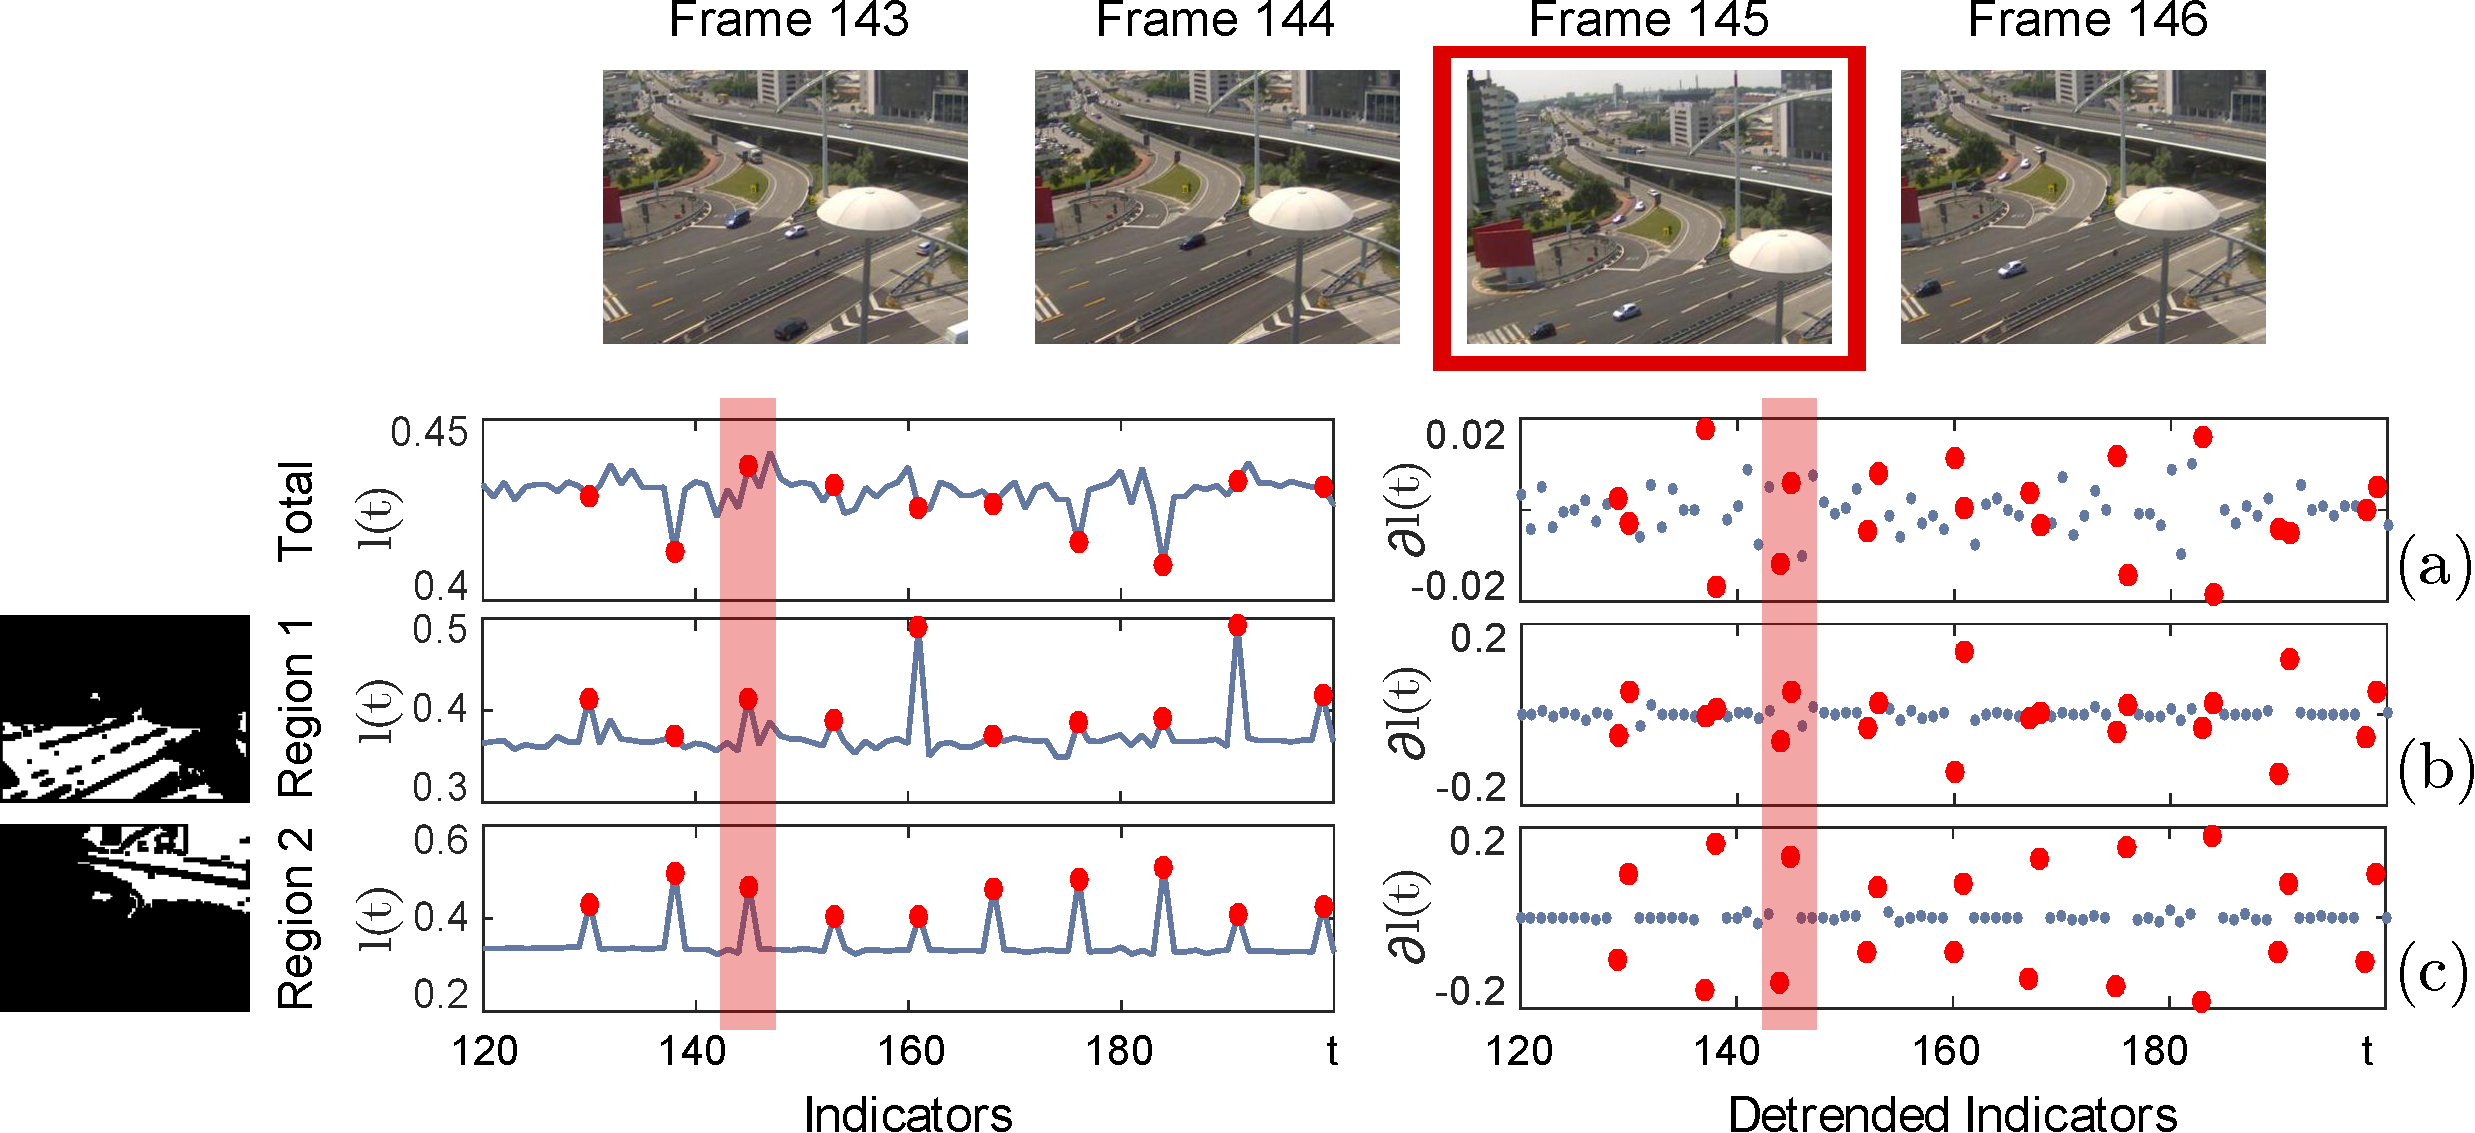
\includegraphics[width=1\linewidth]{Immagini/indicatori}
\caption{Example of camera displacement. Left plots report the luma values, while right plots depict the detrended luma: we show both indicators computed over the full image (\textbf{a}) and on two reported regions (\textbf{b} and \textbf{c}). Red stars indicate a single displaced frame, which occurs at $t =157$. Displacement yields a peak in $l$ and two outliers in the sequence of detrended indicators $\partial l$, which can be clearly detected. }
\label{fig:indicatori} 
\end{figure}
%Tampering changes the sequence of indicators:

Figure~\ref{fig:indicatori}(a) shows how a camera displacement affects the image intensities. First of all, we observe that a displaced frame changes $l(t)$ (in this case introducing a peak) which is also visible in the sequences $l_k(t)$ corresponding to the two displayed regions (Figure~\ref{fig:indicatori}(b) and Figure~\ref{fig:indicatori}(c)). Second, we observe that outlier-detection methods~\cite{Chandola2009} based on density estimates or on confidence intervals --that are very efficient to run-- cannot be straightforwardly applied here. In fact, these methods are meant for independent and identically distributed (i.i.d.) random variables, while here indicators follow an unpredictable trend because of changes in the scene or in the illumination. Therefore, we perform a detrending~\cite{Gustafsson2000} of the indicator sequence by a temporal derivative (line~\ref{DISPL-Test5})
\begin{equation}\label{eq:detrending}
 \partial l_k(t) = l_k(t)-l_k(t-1),  \ \ k = 1, \dots, K\,,
\end{equation}
and we similarly define $\partial g(t)$. 

The sequences of detrended indicators are reported in Figure~\ref{fig:indicatori}, and can be suitably monitored by defining the following confidence intervals:
\begin{equation}\label{eq:confidenceRegions}
 [\overline{\partial l}_k(t) - \gamma_l \sigma_{l_k}, \overline{\partial l}_k(t) + \gamma_l \sigma_{l_k}], \ \  k = 1,\dots,K\,,
\end{equation}
where $\overline{\partial l}_k(t)$ denotes the mean and $\sigma_{l_k}$ the standard deviation of $\partial l$ over $R_k$ (lines \ref{DISPL-Tr1} and \ref{DISPL-Tr7}), computed from the tampering-free frames provided for training (i.e. $z_t\,, t = 1, \dots, T_o$) and $\gamma_l >0$ is a tuning parameter. A similar interval is built for $\partial g$ (line~\ref{DISPL-Tr7}). 

During operations, any indicator falling outside its confidence region is considered anomalous (line~\ref{DISPL-Test6}). To raise a camera-displacement alert we require at least $K-1$ indicators $\partial l_k$ to yield an outlier (line~\ref{DISPL-Test8}). This threshold was set to allow a single region not to change, as it typically happens in the sky when the camera is displaced, either horizontally or vertically. In contrast, any outlier in $\partial g$ would yield a blurring alert (line~\ref{DISPL-Test11}).

It is important to remark that tampering yields outliers in the transient of the detrended indicators~\eqref{eq:detrending}: namely, a single tampered frame yield two outliers (as shown in Figure~\ref{fig:indicatori}) and only the first and the last of few consecutive tampered frames yield an outlier in the detrended indicators. This is the reason why detrended indicators are monitored in a one-shot manner, targeting the detection of the first tampered-frame. On the one hand, this one-shot solution can provide prompt detections, and this is particularly important at the low frame-rates we consider. On the other hand, one-shot monitoring disregards the fact that tampering might persist over several frames. To take this valuable information into account, some form of sequential monitoring should be applied to the indicator sequence as in~\cite{alippi2010detecting}, and possibly combined with the proposed one-shot monitoring.
%
\begin{algorithm}[t]
	% \SetAlgoNoLine
	\LinesNumbered
	\SetAlgoNlRelativeSize{0}
	\SetNlSty{small}{}{.}
	\textbf{Input}: $\gamma_l, \gamma_g$, $\{z_t, t = 1, \dots, T_{0}\}$, $\{R_k, \ k=1,\dots,K\}$ \\
	\textbf{Configuration}:\\
	\lnl{DISPL-Tr1} Compute $\partial l_k(t)$ and $\partial g(t), t = 1, \cdots, T_o$\\ 
	\lnl{DISPL-Tr7} Compute $\overline{\partial l}_k$, $\overline{\partial g}$, $\sigma_{l_k}$ and $\sigma_{g}$.\\
	
	\textbf{Operational phase}:\\
	\lnl{DISPL-Test1} \For{$t=T_{o} + 1,\dots,\infty$}{
		\lnl{DISPL-Test2} Get frame $z_t$, set $n_l =0$;\\
		\lnl{DISPL-Test4} \For{$k=1,\dots,K$}{
			\lnl{DISPL-Test5} Compute $\partial l_k(t)$\\
			\lnl{DISPL-Test6} \If{$\partial l_k(t) < -\gamma_l \sigma_{l_k} \vee \partial l_k(t) > \gamma_l \sigma_{l_k} $}{
				\lnl{DISPL-Test7} $n_l=n_l+1$\\
			}
		}
		\lnl{DISPL-Test8} \If{$n_l\geq K-1$}{
			\lnl{DISPL-Test9} tampering (probably displacement or occlusion) has occurred in $z_t$ \\
		}
		\lnl{DISPL-Test10} Compute $\partial g(t)$\\
		\lnl{DISPL-Test11} \If{$\partial g(t) < -\gamma_g \sigma_{g} \vee \partial l(t) > \gamma_g \sigma_{g} $}{
				\lnl{DISPL-Test9} tampering (probably blurring) has occurred in $z_t$ \\
								}
	}   
	\caption{The Proposed Tampering-Detection Algorithm}
	\label{alg:DISPL}
\end{algorithm}
%
\subsection{Scene Segmentation}\label{subsec:Segmentation}
Scene has to be preliminarily segmented to define regions that our algorithm takes as input (see Algorithm \ref{alg:DISPL}). To this purpose, we use part of the training frames before $T_0$ to compute a feature vector $\textbf{f}(x)\in \mathbb{R}^5$ for each pixel $x\in\mathcal{X}$ 
\begin{equation}
\label{eq:featureVector}
\textbf{f}(x)=\left[r(x);c(x);\bar{l}(x);\sigma_{l}(x);\overline{g}(x);\sigma_{g}(x)\right]\,, \ \forall x \in X\,.
\end{equation}
In \eqref{eq:featureVector}, $r(x)$ and $c(x)$ denotes the row and column of $x$, respectively, $\bar{l}(x)$ and $\sigma_{l}(x)$ the mean and standard deviation of the intensity at $x$, computed over time, and $\overline{g}(x)$ and $\sigma_g(x)$ the mean of gradient norm and its standard deviation, computed overtime. These feature vectors are meant to cluster pixels in regions having similar spatial appearance and temporal behavior over training frames.

Segmentation consists in clustering the feature vectors~\eqref{eq:featureVector} over the whole image by a weighted k-means~\cite{kottke1994motion}. In particular, since the components of the feature vector span very different ranges, we compute the distance between a feature vector and a cluster centroid by scaling the Euclidean distance of a weight inversely proportional to the standard deviation over the cluster. %\gi{Adriano, controlla bene}
%The number of clusters is defined by the Calinski-Harabasz criterion~\cite{calinski1974dendrite}, which initializes the weighted k-means using different number of clusters, and then chooses the best one according a cost function\gi{Adriano controllare come lo chiama}. 
The number of clusters is defined by initializing the weighted k-means using different number of clusters and then choosing the best solution according to the Calinski-Harabasz criterion~\cite{calinski1974dendrite}.

Finally, morphological image-processing operations are executed to remove boundaries between different regions, and eventually regions that are too small. This defines the regions $\{R_k\,, \ k=1,\dots,K\}$, and two examples are reported in Figure~\ref{fig:indicatori}.

\subsection{Computational Complexity}\label{subsec:coputationalComplexity}

The most computationally demanding operations of Algorithm \ref{alg:DISPL} consists in computing of the indicators $g(t)$. Assuming that derivatives in~\eqref{eq:normaGradiente} are computed by the Sobel filters, this requires $34$ operations per pixels\footnote{Execution times can be however  decreased whether hardware implementations of the FFT transform are available}. Computing $l(t)$ requires 1 operation per pixel and the outlier detection over the indicators require two comparisons per frame. Thus, monitoring regions has a negligible impact over the overall computational complexity. 
Segmentation has not been here considered because it is executed only during the initial training phase, and can be performed on an external device connected to the smart camera during configuration.

%FRAME DIFFERENCE:
%\begin{equation}
%	\label{eq:frameDiffReg}
%	\varphi^k(t) = \frac{\sum_{x \in R_k}(z_t(x) - z_{t-1}(x))^2}{|R_k|}, k=1,\dots,K.
%\end{equation}
	

%\begin{algorithm}[tp]
%	% \SetAlgoNoLine
%	\LinesNumbered
%	\SetAlgoNlRelativeSize{0}
%	\SetNlSty{small}{}{.}
%	\textbf{Configuration}:\\
%	\lnl{DEF-Tr0} Extract regions $\{R_k\}, k=1,\dots,K$  \\
%	\lnl{DEF-Tr1} \For{$t=1,\dots,T_{o}$}
%	{	\lnl{DEF-Tr2} Acquire frame $z_t$ \\
%		\lnl{DEF-Tr2a} \For{$k=1,\dots,K$}{
%			\lnl{DEF-Tr3a} Compute $g^k(t)$, $\frac{\partial g^k}{\partial t}(t)$ for the region $R_k$\\
%		}
%		\lnl{DEF-Tr3} Compute $g(t)$, $\frac{\partial g}{\partial t}(t)$ \\
%	}
%	\lnl{DEF-Tr6a} \For{$k=1,\dots,K$}{
%		\lnl{DEF-Tr7a} Define thresholds $\Gamma_{min}^k$ and $\Gamma_{max}^k$\\
%	}
%	\lnl{DEF-Tr5} Define CDT parameters on $g(t)$ variance\\
%	\textbf{Operational phase}:\\
%	\lnl{DEF-Test1} \For{$t=T_{o},\dots,\infty$}{
%		\lnl{DEF-Test2} Acquire frame $z_t$ \\
%		\lnl{DEF-Tr3b} Compute $g(t)$, $\frac{\partial g}{\partial t}(t)$ \\
%		\lnl{DEF-Test2a} $n=0$\\
%		\lnl{DEF-Test4a} \For{$k=1,\dots,K$}{
%			\lnl{DEF-Test5a} Compute $g^k(t)$, $\frac{\partial g^k}{\partial t}(t)$ for the region $R_k$\\
%			\lnl{DEF-Test6a} \If{$\frac{\partial g^k}{\partial t}(t) < \Gamma_{min}^k \vee \frac{\partial g^k}{\partial t}(t) > \Gamma_{max}^k $}{
%				\lnl{DEF-Test7a} $n=n+1$\\
%			}
%		}
%		\lnl{DEF-Test81} \If{$n \geq K-1$}{
%			\lnl{DEF-Test91} $z_t$ is a defocused frame\\
%		}
%		\lnl{DEF-Test8} \If{CDT detect a change on $g(t)$ variance}{
%			\lnl{DEF-Test9} $z_t$ is a defocused frame\\
%		}
%	}   
%	\caption{Blur detection algorithm}
%	\label{alg:DEFOCUS}
%\end{algorithm}

%\gi{Adriano: inserisci qui l'algoritmo e traducilo in inglese. Se riusciamo lo spostiamo prima di tutte le sottosezioni}
\vspace{-0.2cm}
\section{Experiments}\label{sec:experiments}
Experiments are meant to show the effectiveness of the proposed algorithm on real-world sequences, and to specifically assess the advantage of using segmentation for detecting camera displacements. 
\vspace{-0.3cm}
\subsubsection{Considered Methods}
As far as camera-displacement is concerned, Algorithm \eqref{alg:DISPL} is compared against three variants: 1) monitoring the luma on the whole image (\emph{Luma-Total}), 2) monitoring the total energy of the difference between two adjacent frames (\emph{Frame Difference}), and 3) monitoring the luma on $K$ regions obtained by clustering $[r(x), c(x)]$, which yields a Voronoi partitioning of the scene (\emph{Luma-Voronoi}). Frame difference is considered as a baseline technique for displacement detection, while comparison against \emph{Luma-Voronoi} shows the advantages of setting regions depending of the image content. \\
In the experiments on blurring detection, we compare Algorithm \ref{alg:DISPL} (where $\partial g$ is monitored on the whole image), against monitoring $\partial g$ separately in image regions, as done for $\partial l_k$.
\vspace{-0.3cm}
\subsubsection{Datasets}
The considered dataset contains  sequences of  frames taken from webcams monitoring urban areas (e.g., see Figure \ref{fig:sequences}(a)), in which we've taken the central crop of each image (about $3/4$ of the original image). 
%The second dataset was recorded using a Raspberry Pi Model B+ \cite{raspberry} mounting a camera module. 
In order to have a wide and sound dataset, the tampering events have been made synthetically, blurring the frames by gaussian kernels (see, Figure \ref{fig:sequences}(b)) or moving the crop of the frames in order to simulate displacements (see Figure \ref{fig:sequences}(c)). 
%Few sequences of the first dataset contain real tampering events  (Figure \ref{fig:indicatori}). 
%In the second dataset, tampering was introduced by moving the device or spraying water on the camera lens. 
At last we have considered $8$ different scenarios, for a total of $24410$ frames considered, in which we've inserted $5\%$ of displacement events ($1224$ frames) and $5\%$ of blurring events ($1224$ frames).\footnote{Sequences can be released upon request}
\vspace{-0.3cm}
\subsubsection{Performance Assessment}
The typical figure of merit for assessing detection performance in one-shot monitoring methods are the Receiver-Operating Characteristic (ROC) curves: in our case, these can be computed by varying $\gamma_l$, $\gamma_d$ and $\gamma_g$ in a range of values. In particular, each point in the ROC curve depicts a pair of values (1-SPECIFICITY, RECALL) defined as
\[1-\text{SPECIFICITY}_\gamma = \frac{\text{FP}_\gamma}{\text{TN}_\gamma+\text{FP}_\gamma}, \ \text{ and } \ \text{RECALL}_\gamma=\frac{\text{TP}_\gamma}{\text{TP}_\gamma+\text{FN}_\gamma}\]
where TP, FP, TN, FN represent the number of true positives (tampered frames correctly detected), of false positives (tampering-free frames detected), of true negatives (tampering-free frames not detected) and of false negatives (missed tampered frames), respectively, for a given value of $\gamma$.
\vspace{-0.3cm}
\subsubsection{Discussion}
ROC curves and the Area Under the Curve (AUC) reported in Figure~\ref{fig:ROCdisplacement} and its caption indicate that camera displacements can be effectively detected by all the considered methods, and that Algorithm~\ref{alg:DISPL} achieves the best performance (the \emph{Frame-Difference} curve has not been reported because it was quite below the others). This result suggests that separately monitoring the luma over image regions is an effective strategy and that the regions have to be suitably estimated. For the visualization sake, these ROC curves have been reported in a limited range of both axis, and in particular we focus on low values of 1-SPECIFICITY, thus of false alarms. We observe that to achieve a recall of $98\%$, Algorithm~\ref{alg:DISPL} operates at $0.3\%$ of false alarms, which is half of the whole image solution ($0.7\%$) and less than one third of the Voronoi solution ($1\%$). Having few false alarms is important in a low-power context, considering the high number of frames that have to be processed. Most importantly, false alerts are halved basically at no computational overhead.

In contrast, Figure~\ref{fig:ROCdefocus} confirms that when monitoring $g$ it is more convenient to consider the whole scene at once, as typically the regions $\{R_k\}$ do not include the most prominent edge of the scene, which are indeed the most informative part to detect blurring. This is the reason why, in Algorithm~\ref{alg:DISPL}, $g$ is monitored on the whole image.

\begin{figure}[t]
\centering
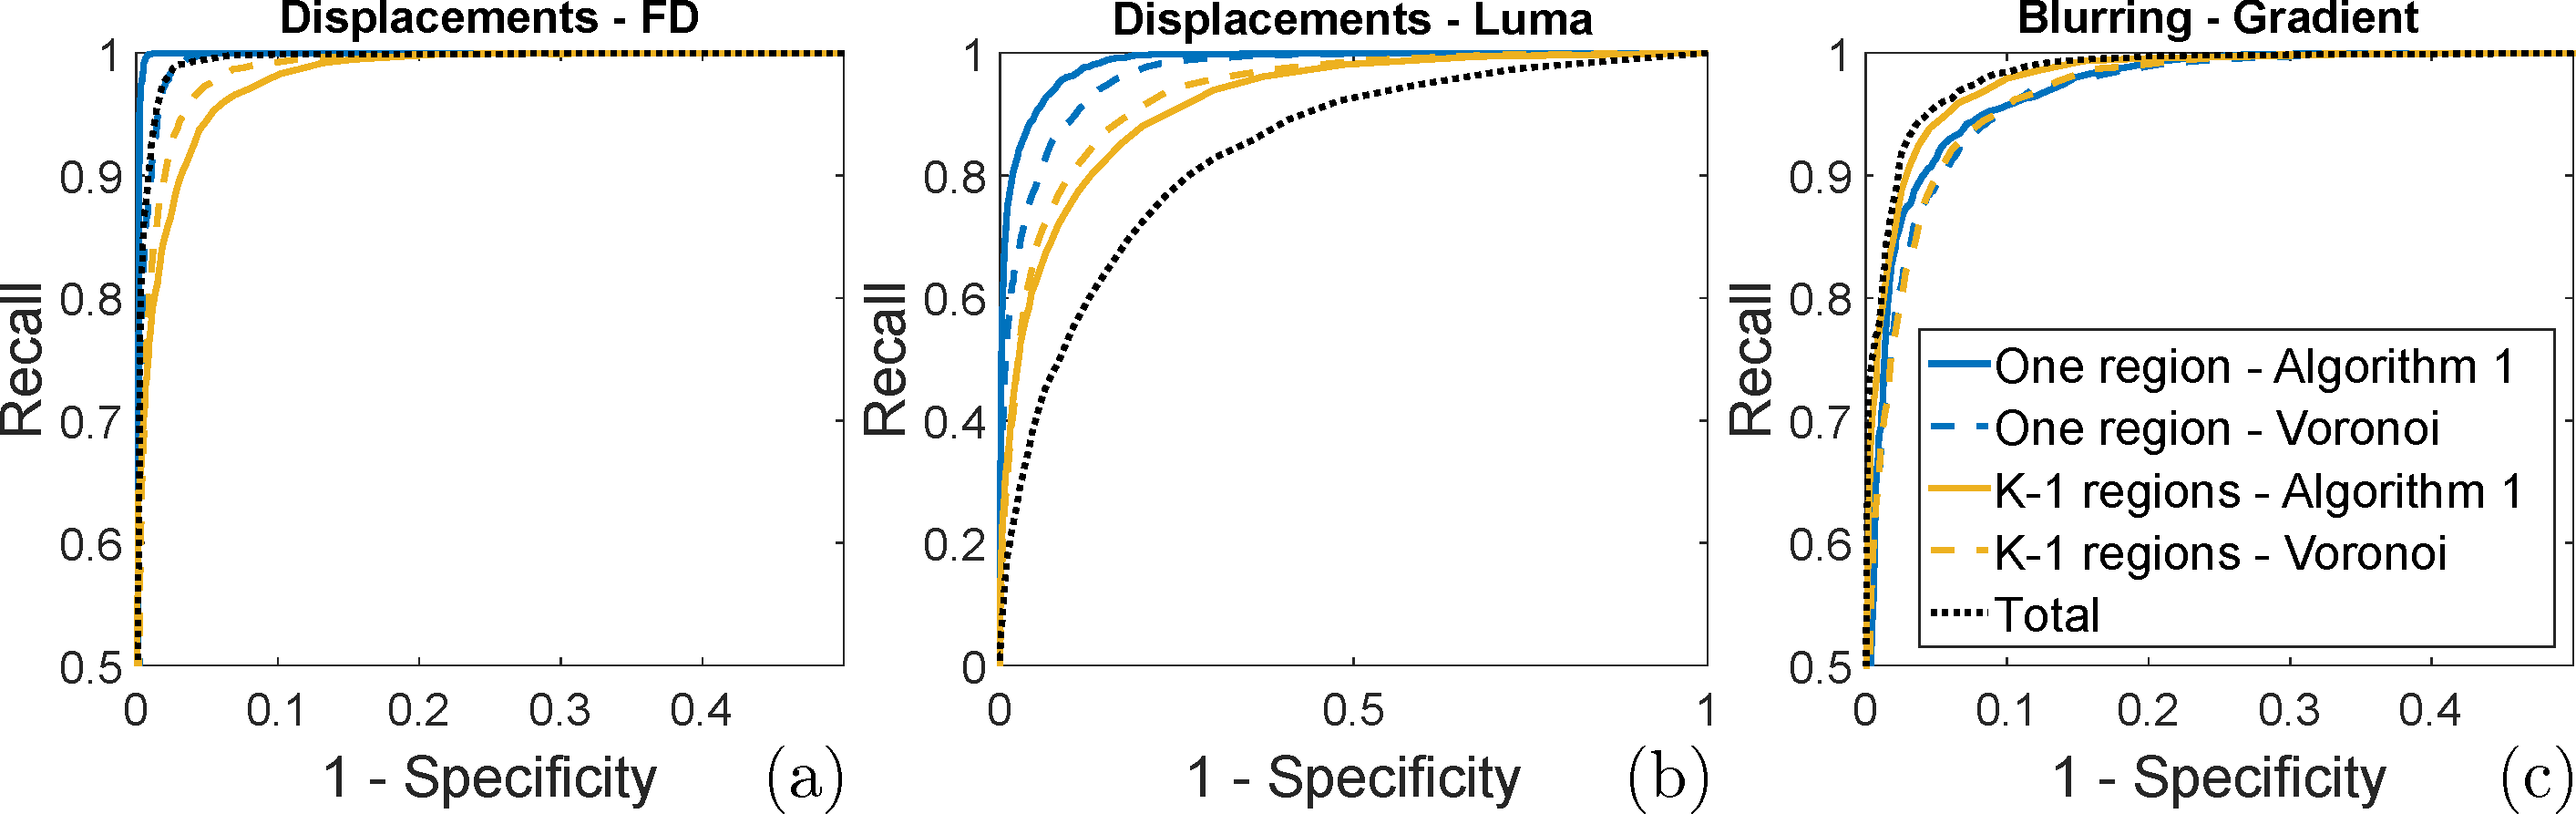
\includegraphics[width=1\linewidth]{Immagini/curve}
\caption{\textbf{(a)} ROC curve for displacement detection.
	%There is an improvement in the performance considering adaptive regions w.r.t. considering the whole image or Voronoi regions.
	The AUC corresponding to Algorithm~\ref{alg:DISPL} (Luma-Region) is $99.94\%$, the AUC of Luma-Total is $99.89\%$ the AUC of Luma-Voronoi is $99.85\%$, and the AUC of Frame-Difference is $99.44\%$ (axis have been zoomed for the visualization sake). Large AUC values indicate that these displacements can be successfully detected and that Algorithm~\ref{alg:DISPL} is the most effective one.
	\textbf{(b)} ROC curve for blurring detection.
	In this case, the Gradient-Total (AUC $99.96\%$) outperforms the Gradient-Regions (AUC $98.95\%$) because this latter do not include the most prominent edges in images, which are the most important information to detect blurring. This is the reason why, in Algorithm~\ref{alg:DISPL}, $g$ is monitored on the whole image.}
\label{fig:ROC}
\end{figure}
%\begin{figure}[htb]
%\centering
%\subfigure[]{\label{fig:buenosAiresDef}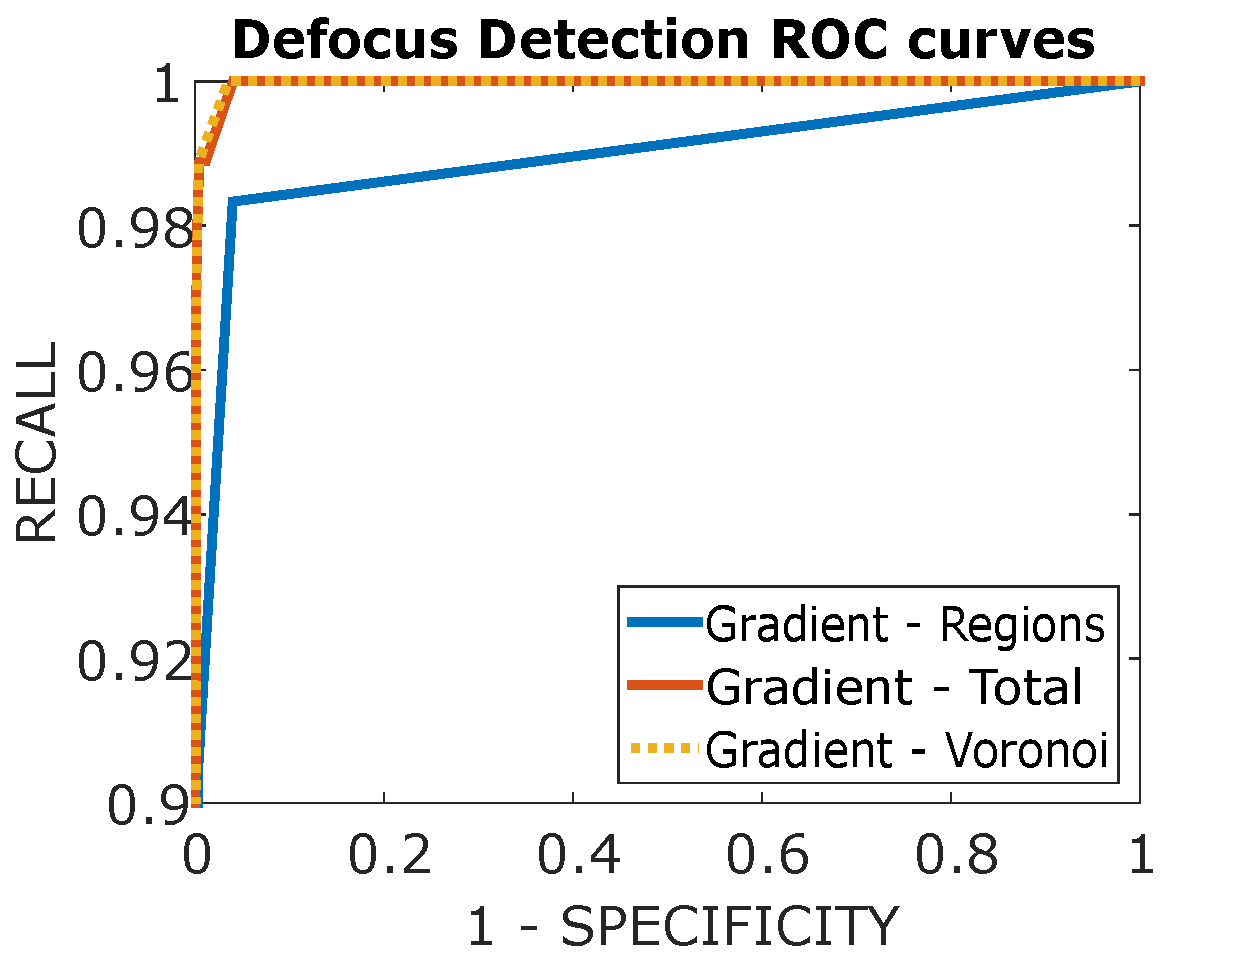
\includegraphics[width=0.45\linewidth]{Immagini/ROCdefocus1}}
%\subfigure[]{\label{fig:buenosAiresDispl} 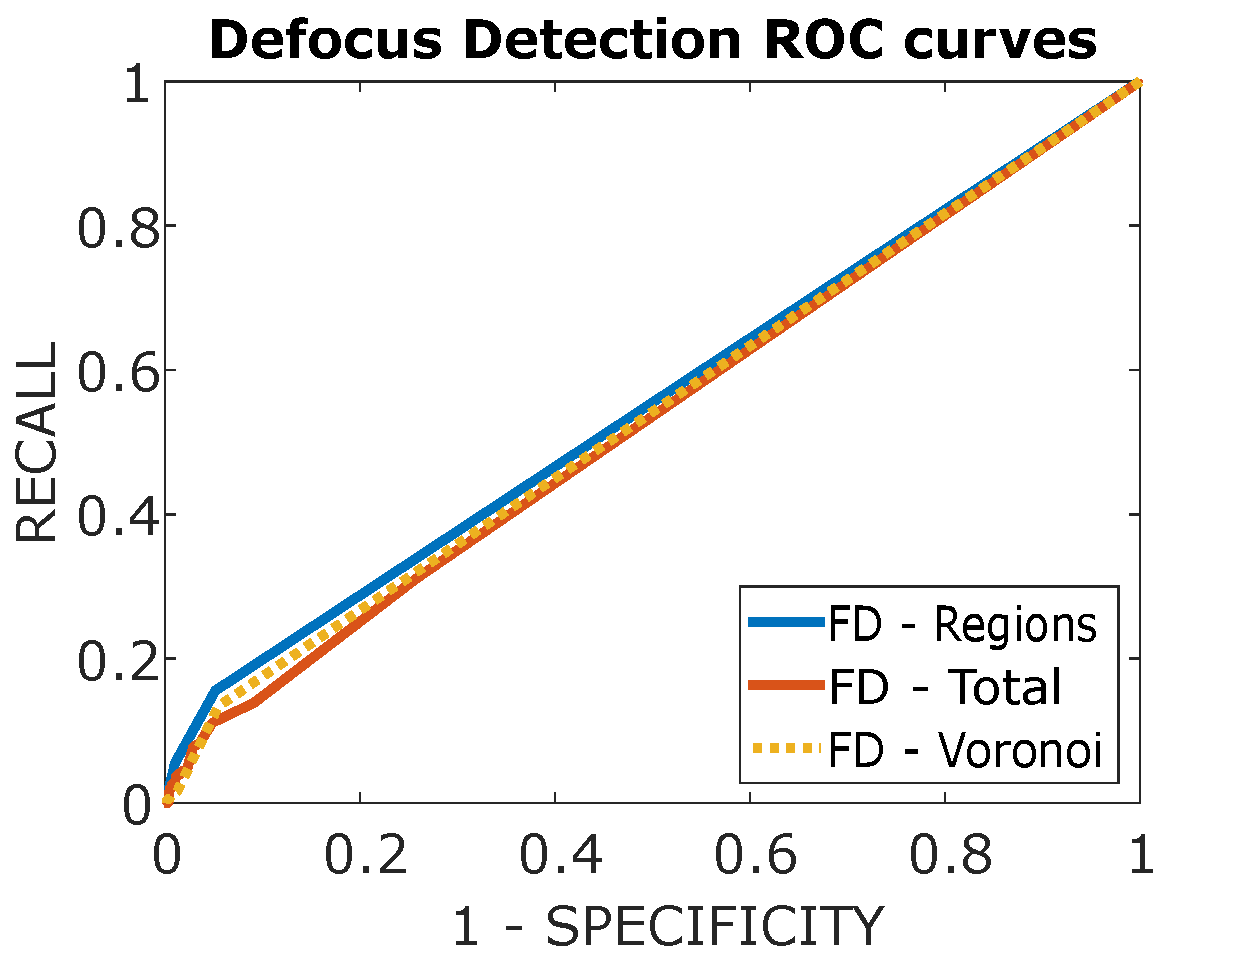
\includegraphics[width=0.45\linewidth]{Immagini/ROCdefocus_fd}}
%\caption{ROC curves for defocus detection, considering three alternative approaches. \textbf{(a)} Analysis of the mean gradient energy. \textbf{(b)} Analysis of the frame differencing.}
%\label{fig:ROCdisplacement}
%\label{fig:ROCdefocus}
%\end{figure}

%
%\begin{table}[tbh]
%\centering
%\begin{tabular}{l|l|l|l|l|l|l|}
%\cline{2-7}
%& \multicolumn{3}{l|}{\cellcolor[HTML]{C0C0C0}\textbf{Displacement Detection}}  & \multicolumn{3}{l|}{\cellcolor[HTML]{C0C0C0}\textbf{Blurring Detection}} \\ \cline{2-7} 
%& \cellcolor[HTML]{EFEFEF}\textbf{Regions} & \cellcolor[HTML]{EFEFEF}\textbf{Total} & \cellcolor[HTML]{EFEFEF}\textbf{Voronoi} & \cellcolor[HTML]{EFEFEF}\textbf{Regions} & \cellcolor[HTML]{EFEFEF}\textbf{Total} & \cellcolor[HTML]{EFEFEF}\textbf{Voronoi} \\ \hline
%\multicolumn{1}{|l|}{\cellcolor[HTML]{EFEFEF}\textbf{Luma}}     & 0.9994 & 0.9989 & 0.9985  &            &            &             \\ \hline
%\multicolumn{1}{|l|}{\cellcolor[HTML]{EFEFEF}\textbf{Gradient}} &  		 &  		  &             & 0.9895 & 0.9996 & 0.9996  \\ \hline
%\multicolumn{1}{|l|}{\cellcolor[HTML]{EFEFEF}\textbf{FD}}         & 0.9974 & 0.9944 & 0.9974  & 0.5526 & 0.5322 & 0.5391  \\ \hline
%\end{tabular}
%\caption{Area under curve of the analized solutions}
%\label{tab:AUC}
%\end{table}

%Numero di operazioni richieste:
%Calcolo di g(t):
%\begin{itemize}
%\item Norma gradiente: 34 FLOP per pixel
%\item Media delle norme del gradiente
%\end{itemize}
%Calcolo di l(t):
%\begin{itemize}
%\item Media dei valori di grigio
%\item Detrending: 1 FLOP per frame
%\end{itemize}
%Monitoraggio one-shot: 2 confronti
%Monitoraggio sequenziale: 
%Ogni 20 frame
%Calcolo intervalli di confidenza: ~70 FLOP
%Confronto tra intervalli di confidenza: 2 confronti
\vspace{-0.3cm}
\section{Conclusions}\label{sec:Conclusion}
\vspace{-0.1cm}
We presented a tampering detection algorithm that leverages a preliminary image partitioning to improve the detection of camera displacements, and that at the same time can detect blurring. The algorithm has low-computational complexity and is suited for low-power cameras operating at low frame rates.

Ongoing work concern the extension of our solution to other types of tampering, such as occlusions or imaging sensor degradations, as well as the integration of this one-shot technique with sequential monitoring scheme such as~\cite{alippi2010detecting}, to leverage the fact that tampering might last more than one frame in the detection. Moreover, we will investigate different segmentation strategy and test our algorithm on a larger dataset.

%Ongoing work regards the.
%Furthermore, we are investigating strategies to improve the detection performance and reduce the number of \textit{FP}s by combination of our solution with other techniques:
%for example we could use sequential techniques on the features, or integrate the frame analysis with the data extracted from MEMS inertial sensors.   


%Random Toughs:
%\begin{itemize}
%\item Better segmentation
%\item tests on larger datasets
%\item The problem of false alarms, radio module activation
%\item Other tampering attacks like obfuscation (??) which might be due to environmental phenomena such as rain, fog and mist over the camera lenses have to be detected by image analysis methods
%\item Displacement can be perceived by MEMS as well but these device alone are prone to false alarms. Visual inspection is necessary to reduce false alarms
%\end{itemize}

%\section*{Acknowledgments}\label{sec:Acknowledgments}
%Authors would like to thank ST for supporting Adriano Gaibotti.

\bibliographystyle{unsrt}
\bibliography{bibl_tesi}

%\begin{thebibliography}{1}
%	
%	\bibitem{Einstein}
%	A. Einstein, On the movement of small particles suspended in stationary liquids required by the molecular-kinetic theory of heat, Annalen der Physik 17, pp. 549-560, 1905.
%	
%\end{thebibliography}
\end{document}



%
%
%
%\subsection{Indicators}\label{subsec:Indicators}

%\begin{equation}
%\label{eq:gradientRegions}
%\begin{array}{ccc}
%g^k(t)&  = & \mathcal{G}^k[z_t] = \frac{\sum_{R_k}\| \nabla z_t(x) \| _2^2 }{|{R_k}|}\\
%\partial g^k(t) & =& g^k(t)-g^k(t-1) 
%\end{array},
%\end{equation}
%
%In particolare, per il calcolo delle derivate orizzontali  abbiamo utilizzato il seguente filtro $f_h$:
%\[f_h = f \circledast \left[ \begin{array}{rcl}
%1 & 0 & -1
%\end{array}\right], \] 
%mentre per il calcolo delle derivate verticali abbiamo utilizzato il seguente filtro $f_v$:
%\[f_v = f \circledast \left[ \begin{array}{r}
%1 \\ 0 \\ -1
%\end{array}\right], \]
%dove abbiamo indicato con $\circledast$ l'operatore di convoluzione.
%Il filtro $f$, invece, \`e ottenuto tramite un campionamento della \textit{funzione gaussiana} $h$, con media $0$ e deviazione standard $\sigma$
%\begin{equation}
%\label{eq:gaussian}
%h(i,j)=\frac{1}{2\pi\sigma^2}\exp\left(-\frac{i^2+j^2}{2\sigma^2}\right),
%\end{equation}
%e ponendo il valore massimo di questa funzione nel centro del filtro.
%Con questi filtri \`e possibile calcolare la \textit{norma del gradiente} nel seguente modo:
%
%Una volta calcolata la norma del gradiente \`e possibile farne la media come specificato in \eqref{eq:energyGradient}.
%Il risultato finale \`e un indicatore \textit{scalare} per ciascun frame acquisito, che pu\`o essere monitorato per individuare eventi di sfocature. 
%In particolare ci aspettiamo che l'evento di sfocatura provochi un abbattimento del valore di $g$.